\documentclass[letterpaper,12pt,oneside]{article}

\usepackage[utf8]{inputenc}
\usepackage[spanish,es-nodecimaldot,es-tabla]{babel}
\usepackage{graphicx}
\usepackage{array}
\usepackage{natbib}
\bibliographystyle{plain}

\title{TÍTULO DE LA PROPUESTA DE TESIS}
\author{NOMBRE DEL ALUMNO}
\date{MES 2024}

\begin{document}

\maketitle

\section*{Resumen}
Describe de manera inicial la propuesta ¿Cuál es el problema?, ¿Hay alguna solución existente? ¿Cuáles?, ¿Cuál funciona mejor?, ¿Cuáles son las limitaciones de las soluciones existentes?, ¿Cómo espera contribuir?, párrafo de 2000 a 5000 caracteres. Este párrafo debe incluir la justificación y el planteamiento del problema y las contribuciones \cite{phil99}. Se deben incluir referencias \cite{smit54, jame76}.

\section{Objetivos}

\subsection{Objetivo general}
Describe el alcance general de la investigación a desarrollar. El enunciado que expresa el objetivo, siempre escribir como primera palabra un verbo en infinitivo, es decir aquellos con terminaciones ar, er, ir. Responde a las preguntas: ¿Qué se va hacer?, ¿Mediante qué o cómo se va hacer?, ¿Para qué se va hacer?

\subsection{Objetivos particulares}
Precisan las acciones que se llevarán a cabo para lograr el objetivo general. Los objetivos específicos son los resultados y beneficios cuantificables esperados cuando se lleva a cabo una estrategia. Responden a la pregunta: ¿Qué va a lograr cada estrategia?. Deben cumplir los siguientes requisitos: Medibles, que permitan su seguimiento y evaluación. Apropiados a los problemas, Objetivos generales y Estrategias. Temporales, con un periodo de tiempo específico para alcanzarlos. Realistas, es decir, alcanzables, con sentido, desafiantes.

\section{Definición del Problema}
Un planteamiento del problema es un enunciado sobre un problema o asunto vigente que requiere acción puntual para mejorar la situación. El planteamiento del problema explica de forma concisa cuál es la barrera que presenta el problema entre el proceso y el estado actual de las cosas. Este enunciado es completamente objetivo y se enfoca en los hechos del problema, dejando fuera cualquiera opinión subjetiva.Para hacer esto mas fácil, se recomienda que preguntes quién, qué, cuándo, dónde y por qué para crear la estructura de tu planteamiento del problema. Esto facilitará crearlo y leerlo, y hará que el problema sea más comprensible y que tenga solución.

\section{Metodología}
Deberá describir el o los procedimientos científico-metodológicos a seguir para cumplir con los objetivos y metas del proyecto, indicando las técnicas, el diseño experimental y las pruebas estadísticas a utilizar. Se explicarán los procedimientos científicos, tecnológicos, de laboratorio, normas aplicables y análisis estadísticos que se seguirán para cumplir los objetivos y metas del proyecto. 

\section{Inventario de materias/temas de la carrera que se utilizarán para el desarrollo de seminario / tesis}
Lista de materias y temas que impactan en el desarrollo de la tesis propuesta.

\begin{itemize}
    \item Fundamentos de programación
    \begin{itemize}
        \item Resolución de problemas 
        \item Fundamentos para la construcción de código a partir del algoritmo
        \item Paradigmas de programación
    \end{itemize}
\end{itemize}

\section{Índice desglosado de la tesis}
El índice propuesto de la tesis con secciones y subsecciones.

\begin{enumerate}
    \item Introducción
    \item Marco teórico
    \item Análisis del problema
    \item Diseño de solución
    \item Implementación
    \item Resultados y pruebas
    \item Conclusiones y trabajo futuro
\end{enumerate}

\section{Resultados esperados}
Esta sección tiene como objetivo exponer y describir los datos que se espera obtener en tu investigación, para posteriormente interpretarlos y contrastarlos con la teoría, el estado de la cuestión y tu propia investigación. Están íntimamente relacionados con los objetivos, preguntas y/o hipótesis de investigación. 

\section{Cronograma de actividades} 
Se definen actividades a desarrollar, los productos entregables, el periodo de realización, etc. Se enunciarán las actividades por desarrollar durante cada una de las etapas del proyecto, así como los tiempos en que se realizarán. Se recomienda usar una tabla tipo Gantt Chart como la que se muestra en la Fig. \ref{fig:cron}.

\begin{figure}[h]
    \centering
    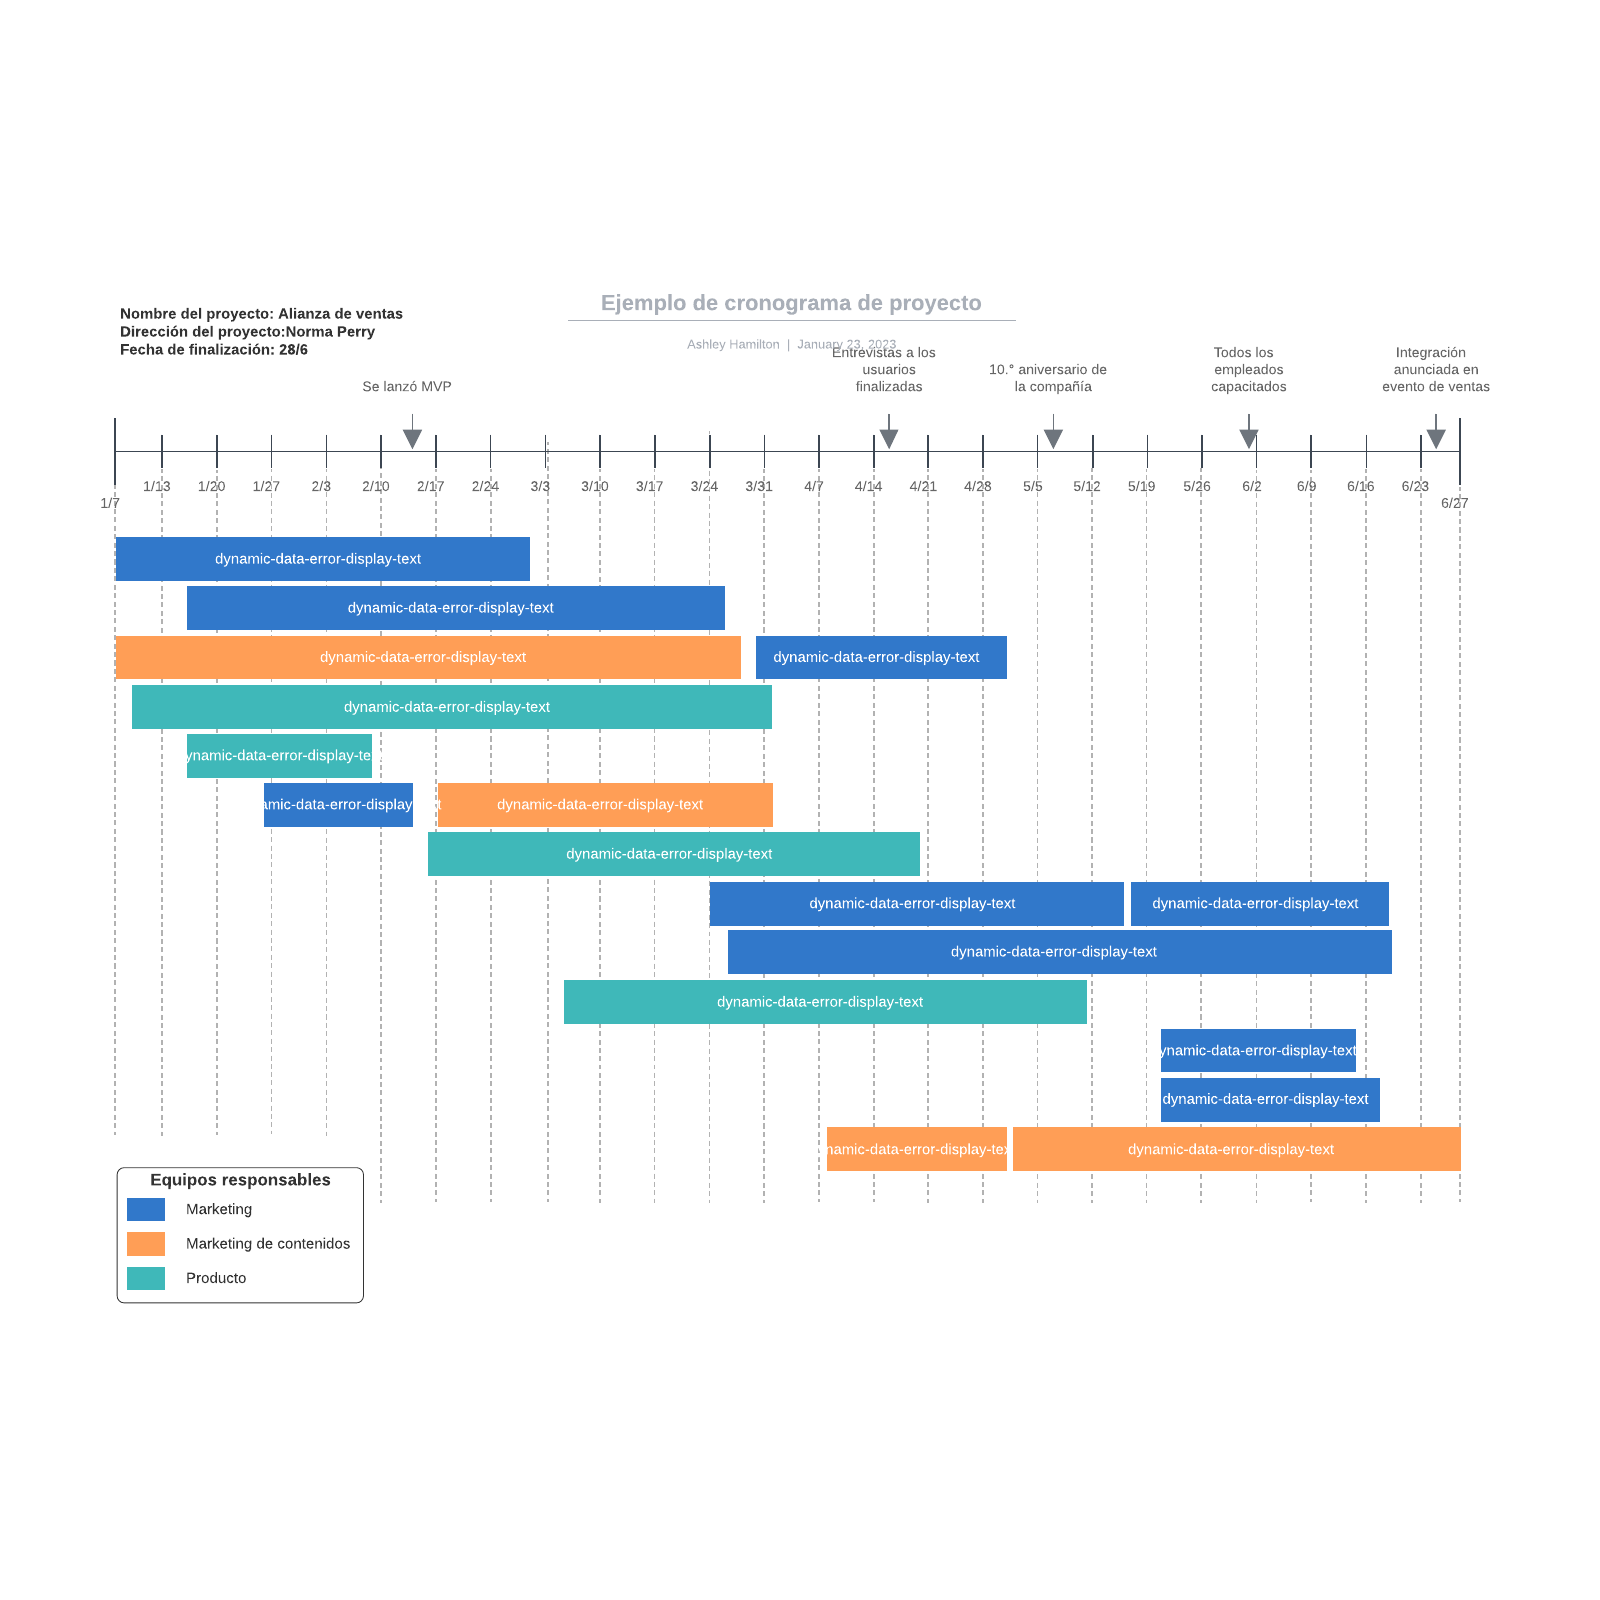
\includegraphics[scale=0.4]{cronograma.png} %Poner el nombre de tu imagen
    \caption{Cronograma de actividades}
    \label{fig:cron}
\end{figure}

\clearpage
\bibliography{mybibliography.bib} %Se asume que se tiene el archivo mybibliography.bib
\end{document}